\chapter{The CMS Detector}
\label{ch:3}

This chapter descriptions the experimental foundation used to measure the $D^0 \to \mu^+ \mu^-$ branching fraction. It begins with a summary of the Large Hadron Collider at CERN, including the injector chain, magnets, running periods, and luminosity profile. 

Then, this chapter describes the CMS detector beginning with a short overview of its geometry and coordinate system before diving into each of its subsystems including the silicon tracker, electromagnetic calorimeter, hadronic calorimeter, superconducting solenoid, and muon chambers. For each of the subsystems, this chapter describes both the basic engineering needed for these detectors and the effect on physics read-out from the detector. 

The next section in this chapter describes how the CMS experiment uses a trigger system to balance the large amount of data with the need to capture sufficient numbers of rare particle interactions. Lastly, this chapter discusses how raw data is reconstructed into particle events and how events are simulated for use in analysis and to benchmark detector response and acceptance. 

\section{The Large Hadron Collider}

The Large Hadron Collider (LHC) at the European Organization for Nuclear Research (CERN) is one of the largest experiments in the world. It has a circumference of 26.7 km, spanning the border of Switzerland and France near Geneva, Switzerland. As the name might suggest, the LHC is a two-ring superconducting hadron accelerator focusing on proton-proton collisions with occasional heavy-ion collision runs. For this thesis, we will entirely focus on proton-proton collisions.

The protons originate from hydrogen atoms and are stripped free using a large electric field. From there, a series of accelerators called the CERN LHC injector chain accelerates the protons to 450 GeV before injecting them into the LHC in bunches. At any given time, there are 39 batches of 72 proton bunches in the LHC with a 25 ns spacing between bunches in a batch to allow for LHC kicker rise time during injection. 

Once injected, the proton bunches are accelerated to a center-of-mass energy of several TeV using two main types of magnets: (i) 1,232 dipole magnets with a field strength of 8.3 T, which bend and accelerate the protons along the circular beam pipes, and (ii) 492 superconducting quadrupole magnets, operated at 1.9\textdegree K, which focus the proton bunches to maintain beam stability.

Once the particles are accelerated to their target energy, they collide at four main interaction points within the LHC. These correspond to the four major LHC experiments: two general-purpose detectors capable of a broad range of physics analysis: ATLAS (A Toroidal LHC Apparatus) and CMS (Compact Muon Solenoid); one detector optimized for heavy-ion collisions: ALICE (A Large Ion Collider Experiment); and one detector focused on $b$-physics: LHCb. Five more smaller experiments exist at secondary sites in the LHC: two specialized in particles that brush past each other, one experiment near LHCb to look for magnetic monopoles, and two experiments near ATLAS specialized in light particles, such as neutrinos. The full CERN accelerator complex can be seen in figure \ref{fig:cern-accelerator-complex}

\begin{figure}[htbp]
    \centering
    \includegraphics[width=0.8\textwidth]{figures/chapter3/CERN-accelerator-complex.png}
    \caption{The CERN accelerator complex \cite{ref:Lopienska}}
    \label{fig:cern-accelerator-complex}
\end{figure}


One of the main difficulties of circular colliders is the rapid loss of every through synchrotron radiation, the electromagnetic radiation emitted when relativistic charged particles move along a curved path. The total power radiated by syncroton radiation in circular colliders is given by
\begin{equation}
    P = \frac{q^2p^4}{6 \pi \epsilon_0 m^4 c^5 r^2}
\end{equation}
where $q$ is the charge of the particles, $p$ is the momentum of the particle, $m$ is the rest mass of the particle, and $r$ is the radius of the collider. This gives the LHC two main advantages in producing high momentum-energy particles without loosing as much power to syncrotron radiation: (i) comapared to electron-positron colliders, such as the LHC's predecessor the Large Electron-Positron collider, the mass of protons is much large and (ii) the radius of the LHC is larger than any other collider in the world. 

Another difficulty of high energy colliders is the rarity of physically interesting collisions. Not only is it difficult to have two protons collide, but it is also rare to have a collision that will get included in an analysis. Due to these factors, the LHC operates at a very high beam intensity, measured as luminosity. The luminosity of of an accelerator is given by
\begin{equation}
    L = \frac{N_b^2n_b f_{rev} \gamma_r F}{4 \pi \epsilon_n \beta^*}
\label{eq:luminosity}
\end{equation}
where $N_b$ is the number of protons per bunch, $n_b$ is the number of bunches per beam, $f_{rev}$ is the revolutuon freuqnecy, $\gamma_r$ is the Lorentz factor, $F$ a geometric factor, and lastly $\epsilon_n$ and $\beta^*$ determine the interaction rate at the interaction point. The high luminosity at the LHC is achieve largely with the $\approx 10^{11}$ protons per bunch. However, this causes an entire host of problems due to the high number of background collisions, which will we discuss further in the next section. 

Instead of running continuously, the LHC breaks up it's data collecting into runs, each at a different center-of-mass energy and luminosity. The first run from 2010-2012 had a 8 TeV ceneter=of-mass energy with a total luminosity of $29.45 \; \text{fb}^{-1}$. Run 2 occurred from 2015-2018 and had a 13 TeV center-of-mass energy with a total luminosity of $163.6 \; \text{fb}^{-1}$. Run 3 started in 2022 and is currently ongoing at a center-of-mass energy at $13.6$ TeV and a targeted luminosity of $42 \; \text{fb}^{-1}$. 

\section{The CMS Detector}

The CMS detector is a large cylindrical detector that almost entirely wraps around the proton beam. It is 21 meters long and 15 meters in diameter, weighing 14,000 tonnes. It is composed of 5 main subsystems wrapped in layers around the beam pipe. These five layers are the silicon tracker, the electromagnetic calorimeter, the hadron calorimeter, and superconducting solenoid, and the muon chambers. These layers are wrapped in layers around the beam line through the center of the detector and can be seen in figure \ref{fig:cms-detector-cutout.png}. More discussion on the subsystems of CMS will proceed in following sections. However, one must first understand the coordinate system.

\begin{figure}[htbp]
    \centering
    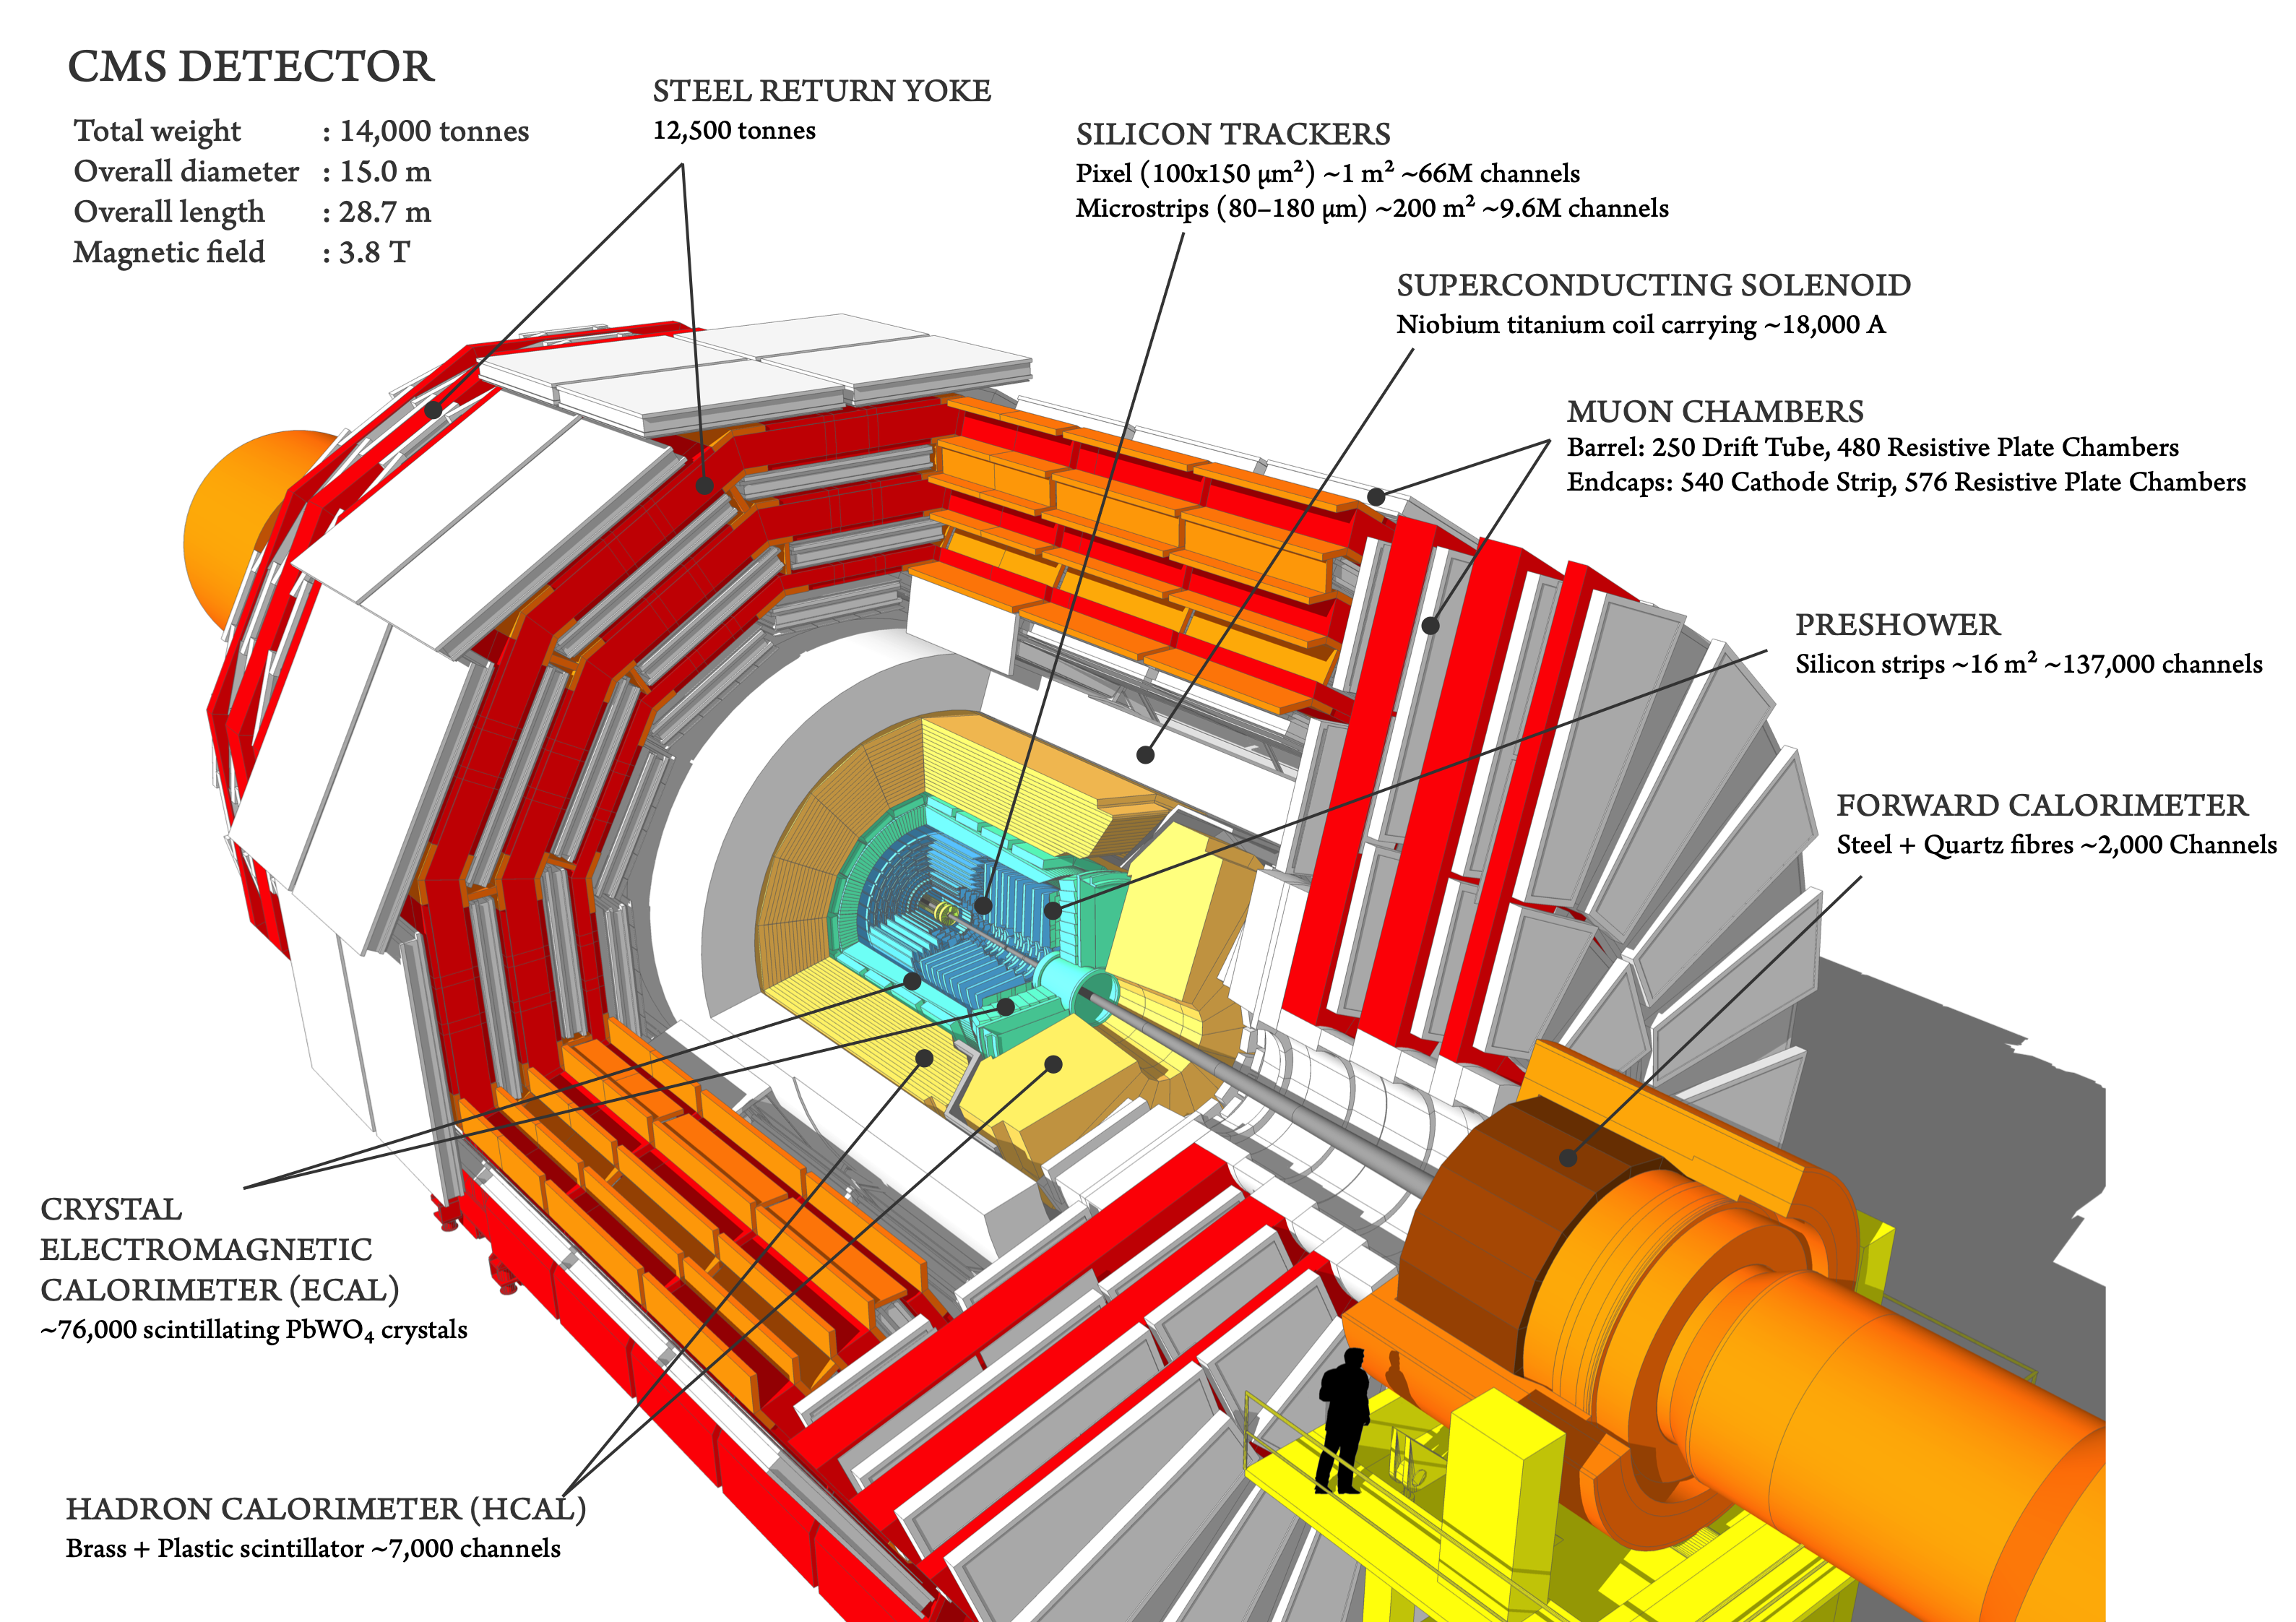
\includegraphics[width=0.8\textwidth]{figures/chapter3/cms-detector-cutout.png}
    \caption{A labeled cutaway diagram of the CMS detector \cite{ref:sakuma}}
    \label{fig:cms-detector-cutout.png}
\end{figure}


The coordinates used in CMS are $\phi, \eta,$ and $r$ with the origin located at the interaction vertex at the center of the cylinder. $r$ represents the distance from the point of the interest to the origin. $\phi$ describes the azimuthal angle along the plane normal to the beam line and is often ignored due to the complete symmetry in $\phi$. Lastly, $\eta$ is known as the pseudo-rapidity, describing the angle of a particle relative to the beam line, $\theta$, as
\begin{equation}
    \eta \equiv -\ln\left[ \tan(\left(\frac{\theta}{2}\right) \right]
\end{equation}
For high energy particles, this is a good approximation of rapidity, given by
\begin{equation}
    y = \frac{1}{2} \ln\left( \frac{E + p_z}{E-p_z}\right)
\end{equation}
where $p_z$ is the momentum along the beam line. This is used instead of the conventional angle $\theta$ because rapidity of particles are invariants under special relativity while the standard angle $\theta$ is not. For example, if two particles have rapidities $y_1$ and $y_2$ and the difference $y_1 - y_2$ remains invariant in any reference frame. The CMS detector has two main regions: the barrel which wraps around the beam pipe and the endcaps which cover the ends of the cylinder. The exact $\eta$ coordinate at which the barrel stops and endcap starts varies by subsystem at CMS, but needs to be carefully considered due to biases introduced because of detector geometry as you move from the barrel to the endcap. 

One other quantity frequently used in describing particle kinematics is $p_T$, or the momentum of the particle transverse to the beam line given by
\begin{equation}
    p_T = |\vec{p}|\text{sech}(\eta)
\end{equation}
The full set of coordinates and the CMS geometry can be seen in figure \ref{fig:cms-coordinate-system}.

\begin{figure}[hb!]
    \centering
    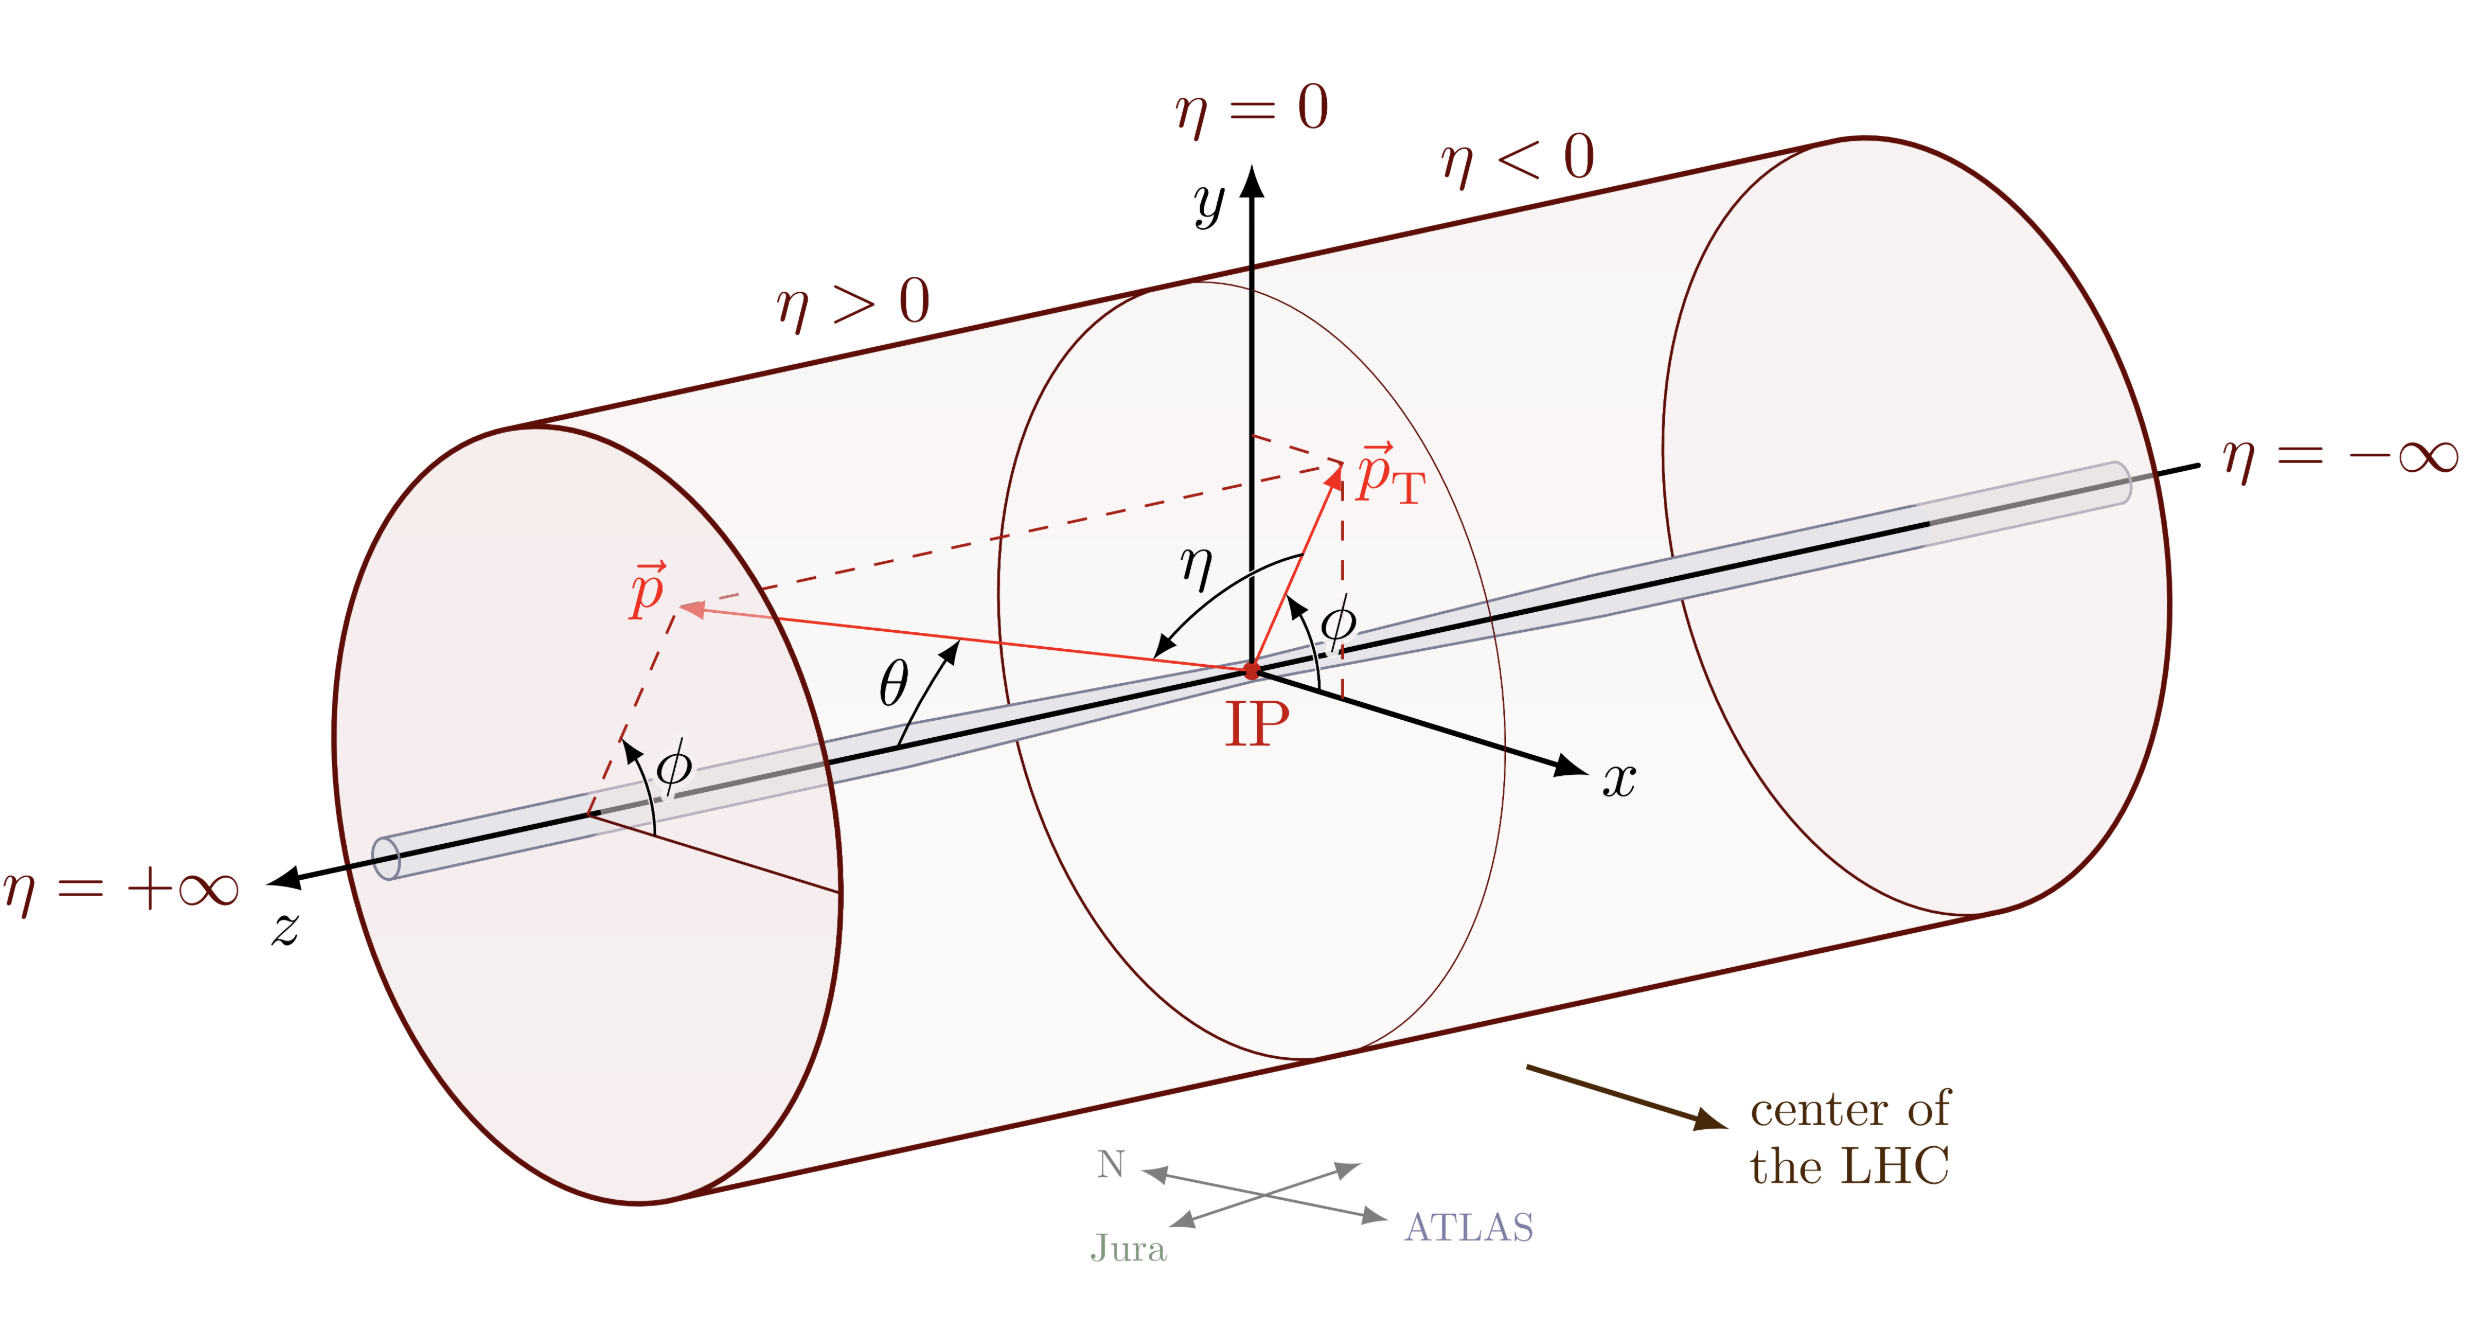
\includegraphics[width=1.0\textwidth]{figures/chapter3/CMS-coordinate-system.png}
    \caption{The CERN accelerator complex}
    \label{fig:cms-coordinate-system}
\end{figure}



\subsection{Solenoid Magnet}

One of the easiest ways to measure the electromagnetic charge of high energy particles is to introduce them into a strong magnetic field and measure the curvature of their tracks. Additionally, the curvature is also dependent on the momentum of the incoming particle, allowing the detector to reconstruct the momentum of charged particles from their tracks. Therefore, the presence of a strong magnetic field across all other subsystem is extremely important. 

The CMS detector contains a 3.8 T solenoid magnet in the middle of the other subsystems. The solenoid is approximately 6 meters in diameter and 13 meters in length, making it one of the largest of its kind ever constructed. Its immense field strength enables CMS to accurately reconstruct the trajectories and momenta of particles produced in collisions, even at very high energies.

\subsection{Silicon Tracker}

Before the tracks of particles can be disturbed by interactions with other detector components, the silicon tracker reconstructs a precise track that demonstrates the particle's trajectory. This is most commonly used for locating their primary vertices, the exactly location of their production, as well as assisting in kinematic reconstruction. In order to do this, silicon is configured in a reverse-biased p-n junction. As charged particle pass through the silicon, they ionize silicon atoms, creating electron-hole pairs. This electric field pushes electrons toward the n-type electrode and hole toward the p-type electrode, causing a current pulse. This current pulse is then read out by Application-Specific Integrated Circuits (ASICs). Due to this process of tracking, it is important to note that the tracker is not able to detect neutral particles. 

The detector is made of two layers of silicon detectors: small pixels located near the center of the tracker and larger strips located near the outside of the detector. The pixels have a size of $100 \times 150 \mu m$, allowing for them to have an extremely fine resultion. Further out, the large strips arranged in a vertical/horizontal pattern reconstruct the track of charged particles by superimposing the vertical and horizontal signals. This allows for more precise modeling of the particle's position, but at the cost of resolution. Strips closer to the center of the detector are smaller while strips further outside are larger. 

\subsection{Electromagnetic Calorimeter}
A calorimeter is any device that measures the heat exchanged between a process and its environment.  In particle physics detectors, the term takes on a specialized meaning: it denotes a system that destructively measures a particle’s energy by scattering it in dense material and recording the ensuing shower.  Such devices therefore contain two essential components: (i) a passive absorber, which initiates the shower, and (ii) a scintillating medium, which converts the energy released by the shower into optical photons that can be read out.

Perhaps the most common example of a calorimeters is the electromagnetic calorimeter (ECAL), whose purpose is to stop and measure high‑energy electrons and photons.  Incoming $\gamma/e^{\pm}$ particles lose energy almost exclusively through well‑understood QED processes such as bremsstrahlung and pair production, causing a cascade to lower energy photons and electrons, causing an electromagnetic shower such as in figure \ref{fig:electromagnetic-shower}. Eventually the cascaded photons and electrons have a low enough energy that they are able to be easily absorbed and measured by the scintillator.  The characteristic scale of this shower is the radiation length~$X_{0}$, the mean distance over which an electron’s energy is reduced by a factor~$e^{-1}$.  In practice an ECAL is built to a depth of $\sim\!20$–30\,$X_{0}$ so that the entire shower is contained. The other important scale is the Molière radius, or the radius of the cylinder containing $90\%$ of the shower's energy.

\begin{figure}[htbp]
    \centering
    
\includegraphics[width=0.4\textwidth]{figures/chapter3/electromagnetic-shower.png}
    \caption{A schematic example of an electromagnetic shower caused by bremmstrahlung and pair production.}
    \label{fig:electromagnetic-shower}
\end{figure}

In CMS the ECAL is a homogeneous calorimeter, meaning the absorber and the scintillator are the same material (lead‑tungstate, PbWO$_4$) so that virtually no energy is lost to passive absorbers since they are the same as the scintillator. Additionally, homogeneous calorimeters allow for the same response from every angle due to their homogeneity. The barrel section ($|\eta|<1.48$) and two end‑caps ($1.48<|\eta|<3.0$) together comprise 75,848 crystals, each $22\times22\;\text{mm}^2$ at the front face and $230\;\text{mm}$ long ($25.8\,X_{0}$). The fast scintillation time of PbWO$_4$ ensures that $\sim80\%$ of the light is collected within a single LHC bunch crossing, and the small Molière radius ($R_M\simeq21$ mm) localizes showers largely inside one crystal.  

Radiation damage gradually darkens the crystals. Therefore, CMS injects laser light between fills to monitor transparency and applies time‑dependent calibration constants. This careful calibration allows for precise reconstruction of an electromagnetic particle's energy. 


\subsection{Hadronic Calorimeter}
While the ECAL measures purely electromagnetic showers, the hadronic calorimeter (HCAL) captures and quantifies the energy of neutral and charged hadrons.  The underlying physics is much more complex. When an incoming hadron interacts strongly with the passive absorber of the HCAL, it produces a hadron shower. The hadrons in the shower then produce electrons and photons in three main ways: (i) through neutral pions which decay to charged kaons or protons, which interact to produce two photons through a 3 vertex feynman diagram, (ii) through charged hadrons ionizing the passive absorber, and (iii) through evaporation and spallation of the nuclei of the passive absorber. Then, these photons and electrons produce showers which are measured, similar to the ECAL. While neutral pion decay accounts for most of the energy converted to electromagnetic showers, the specific fraction of hadron energy that is converted to photon/electron energy is highly dependent on the incoming hadron’s momentum and energy. This leads to a lower energy resolution compared to ECALs since it is difficult to estimate how much energy is not converted to photons and electrons. Additionally, because of the addition of hadron showers in HCALs, the radiation length of the HCAL is longer, leading to a larger detector compared to ECALs. 


CMS uses a sampling HCAL.  Alternating layers of passive brass absorber and plastic scintillator tiles form a barrel ($|\eta|<1.3$), two end‑caps ($1.3<|\eta|<3.0$), and a forward calorimeter extending to $|\eta| < 5.2$. Radiation and aging also affect HCAL response, similar to ECALs. CMS calibrates the system continuously using embedded radioactive sources, dedicated laser/LED pulses, and $\phi$‑symmetry methods.

\subsection{Muon Chambers}

Lepton detection is critical to many anylsis performed at CMS, including this one, which focuses on muon and electron final states. Neutrinos are too light to be detected by anything in the detector and $\tau$ leptons are so unstable they always decay into other products which we measure. Electrons are well measured in the ECAL, but muons are heavy enough that they almost always don't get absorbed by the ECAL and therefore are not detected. Therefore, there is a need to construct large muon chambers, specifically built to detect muons. 

The muon chambers work by measuring the muon's track as it leaves the detector. The magnetic field is still strong enough that the momentum  and sign of the charge of the muon can directly be reconstructed from the curvature of the track. In this way, the muon chambers can be though of as very large trackers. 

There are three different types of gaseous detectors used in the muon system: drift tubes, cathode strip chambers, and resistive plate chambers. The drift tubes are 4cm wide tubes containing a positively charged stretched wire and a gas volume. When muons interact with the gas, they release electrons which drift toward the positively charged wire, causing a measurable pulse on the wire. Due to the length of the wires, drift tubes work very well in environments with uniform magnetic field and a low muon rate and are therefore found at the barrel. Cathode strip chambers contain an array of positively charge wires arranged in a grid. They work similarly to drift tubes, but the array allows for better measurements in the high muon rate and magnetic field variation environment of the endcap. Lastly, resistive plate chambers are gaseous parallel-plate detector consisting of one positively charged and one negatively charged plate. While they operate similarly to drift tubes and cathode strip chambers, the have detecting strips instead of wires to measure the electrical signal of released electrons. This produces a much more precise time resolution but a fairly poor spatial resolution. Therefore, these detectors are present throughout the barrel and the endcap, complementing the drift tube and cathode strip detectors to improve the timing resolution of the muon chambers. 




\section{Triggers}
\label{sec:triggers}

As mentioned earlier, high energy colliders are faced with the problem that collisions that are interesting for physics analysis are rare. This results in a need for a very high rate of data production and a large amount of background. 
At the LHC, bunch crossing happen every 25 ns and result in an average of 20 collisions. Processing a storing the data from all these collisions is not technologically possible. Therefore, a trigger system is built to "trigger" on interesting physics events while ignoring all others. This trigger reduces the event rate from 800 MHz to roughly 1 kHz. The quality of data output requires a computing farm running advanced algorithms, known as the High Level Trigger (HTL). However, the raw data rate is too large to give to any computer and must therefore be filtered by hardware, forming the Level-1 (L1) trigger. The L1 trigger reduces the event rate to 100kHz, where it can be processed by the HLT. % TODO should probably include this citation:  M. Tosi, “The CMS trigger in Run 2,” Tech. Rep. CMS-CR-2017-340, CERN, Geneva, Oct 2017.

The L1 trigger is entirely built on Field Programmable Gate Arrays (FPGAs), custom integrated circuits that can be configured even after manufacturing, allowing for CMS to tune its hardware triggers without replacing hardware. These L1 triggers are segregated in terms of detector sub-systems, meaning that they only trigger once an interesting ECAL energy deposit has been found, an interesting muon detecetion, etc. but not on the event as a whole. 

In contrast to the L1 trigger, the HLT is a large computing center with over 30,000 cores. One of the most important features of the HLT are the large arrays of buffers that are able to hold information before or while the HLT processes it, ensuring that the HLT has enough time to consider the event as a whole. The HLT system can be abstracted as a series of paths that each specialize in a type of event. For example, one might be interested in dimuon events with high muon energy. Carefully selecting the trigger paths is one of the most important aspects of any analysis. 

One of the largest difficulties that come with using triggers is avoiding the bias that comes with picking a specific HLT trigger path. Numerous methods are used to prevent large trigger bias in analysis, including normalization channels and measuring trigger efficency across whatever variable you are interested in. To allow these calculations to occur, a MinBias dataset is created, which is a random small sample of the raw data read out. A discussion on the triggers used for this analysis and their bias can be found in section ??% TODO: insert section name here. 

\section{Event Reconstruction}

\subsection{Electrons}

\subsection{Muons}

\subsection{Jets}

\section{Similation Data}

TODO: not sure if I need to write about this